\subsubsection*{Design}
As seen in \cref{img:coredes} the core will of the previously described functions, a connection to the frame buffer, and a connection to a VGA interface.

The graphic accelerator has a double frame buffer. It keeps track of the information of two separate frames. One of the frames is drawn by the VGA module, the other is being created by the graphics accelerator and CPU. The data for the objects are moved into the RAM of the CPU.

As some functions of the Blitter correlate with the functions of the ALU\cite{data1988amiga}, the two blocks will be merged together. In the following the two of them will be referred to as the ALU. This part of the core will either write directly into the frame buffer or it will delegate the drawing to the proper function core. These smaller function cores consist of the basic graphical primitives, as discussed in \cref{subsec:des_bresenham}.
\begin{figure}[H]
	\centering
	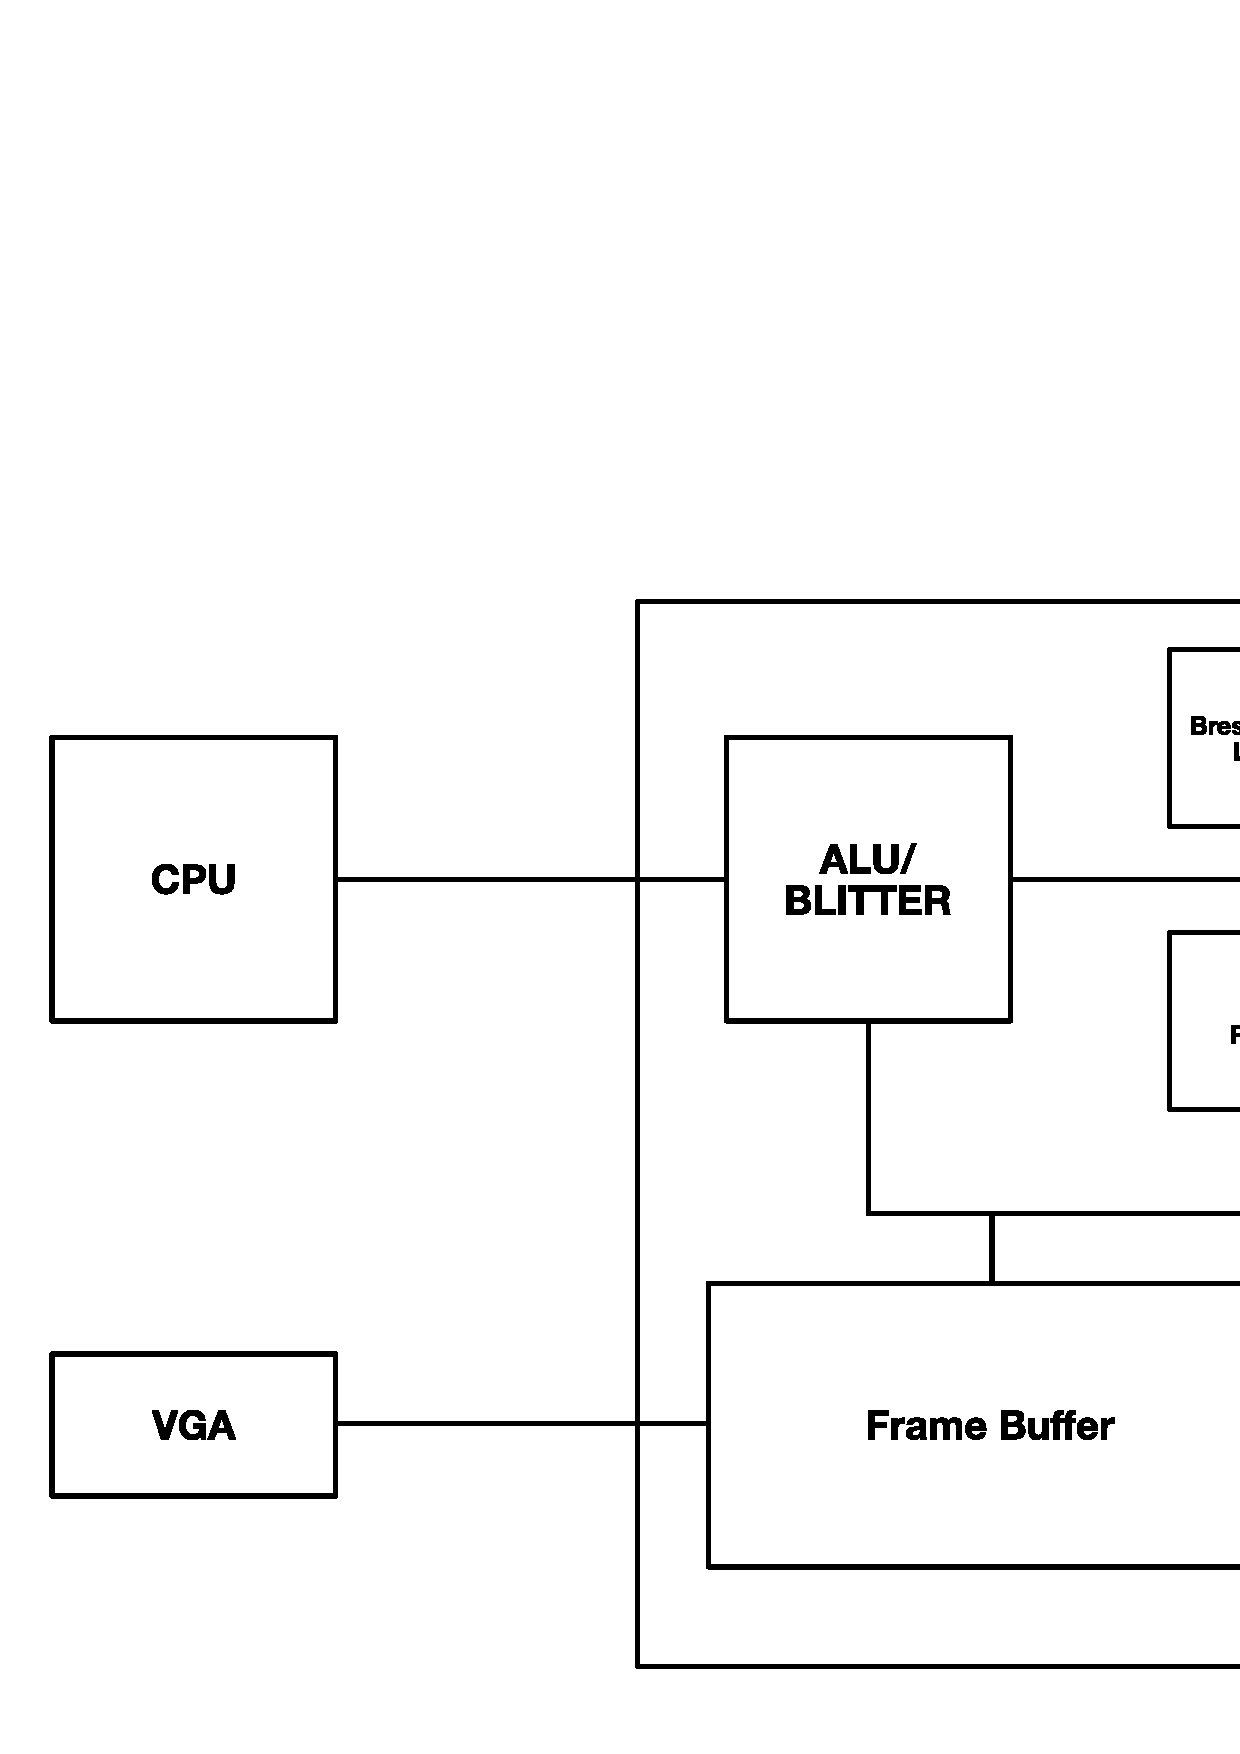
\includegraphics[width=0.65\textwidth]{coredesign}
	\caption{Graphical Design of the AEGIS Core }
	\label{img:coredes}
\end{figure}

For the communication between the CPU and the graphics accelerator, we use two AXI4 buses. The first one is a Axi4Shared for the communication with the CPU, and the second one is a Axi4ReadOnly for the communication with the RAM.

When a write command is send over the AXI4 bus, the graphics accelerator looks at the address. Is the address in the range of the double frame buffer, it is going to write to it. Otherwise the address determines, what the graphics accelerator has to do. Further data for operation is obtained from the memory at the address from the data value.

\subsubsection*{Implementation}
The core of the graphics accelerator can be found in the file \texttt{MCP}. Because we need to connect it with the RISCV and need extra memory, the core is connected to two AXI buses. The first one being a shared bus with the RISCV as a slave, while the second one is one to a read-only bus for the additional memory as a master.

As the cores logic is higher in complexity we needed to use two state machines, with one being the main state machine and the other being nested in the first. The idle state of the main state machine waits until the shared AXI bus the valid command is set. This can be seen in \cref{idlecore} on line 4. After that we have to check if the AXI bus wants to read or write. When the \(\text{25}^{\text{th}}\) bit is set, we save data from the AXI bus and continue with the wait state, when that bit is not set the state machine can directly read and write from the frame buffer. The user must keep track which frame buffer they want to read or write to, though.
\begin{lstlisting}[language=scala, caption={Idle State of the core}, label=idlecore]
idle.whenIsActive{
	write := io.axicpu.sharedCmd.write
	id := io.axicpu.sharedCmd.id
	when(io.axicpu.sharedCmd.valid 
		&& (!io.axicpu.sharedCmd.write || io.axicpu.writeData.valid)) {
		when (!io.axicpu.sharedCmd.addr(25)) {
			goto(waitState)
		} otherwise{
			address := io.axicpu.sharedCmd.addr
			raddress := io.axicpu.writeData.data.asUInt
			goto(waitState)
		}
	}
}
\end{lstlisting}
In the wait state, we set the needed AXI bus signals for the handshake described in \cref{subsec:axi} and continues to the response state. Here we set the needed signals for the response and wait until the AXI bus gives its ok. After that it can go into the readdata state or the switch state, depending of if the frame buffer switch is requested.

Before the switch case in the readdata state is running, the nested state machine is activated. This state machine is used for the communication with the memory that is connected via the read-only bus. In this state machine we set the signals for the AXI master bus, this can be seen in \cref{axisetting}. Here we set how big a word is for the burst mode and that we are able to receive data.
\begin{lstlisting}[language=scala, caption={Setting the AXI master bus signals}, label=axisetting]
io.axiram.readCmd.addr := raddress.resized
io.axiram.readCmd.size := B"010".asUInt
io.axiram.readRsp.ready := True
\end{lstlisting}
The read state is then divided into two stages. The first stage gets the signals and the second one saves them into the temporary variables. Internally the second state is also split up into four separate states, because of the different variable needed for the separate functions. Here the sprite state saves the sprite directly into the frame buffer, as discussed in \cref{subsec:des_blit}. When all the data is read, we go into the exit state. This is needed as we are only allowed to exit the state machine from one state and not several.

After the nested state machine is ready the readdata state determines which function we want to execute. After the functions are ready it goes back into the idle state.